\documentclass{article}
\usepackage{graphicx}
\usepackage[margin=1in]{geometry}
\usepackage[outdir=./]{epstopdf}  					% Avoids errors when input figures
\usepackage[labelsep=period,labelfont=bf]{caption}
%\usepackage{subcaption}

\begin{document}
	\begin{figure}[tbph]
		\caption{Comovement of Yield Curves: Connectedness Index} \label{fig:dy_index_ts}
		\begin{center}
			\begin{minipage}{0.9\linewidth}
				\begin{center}
					\begin{subfigure}[t]{\linewidth}
						\includegraphics[trim={0cm 0cm 0cm 0cm},clip,height=0.38\textheight,width=\linewidth]{../Figures/Estimation/dy_index_dn_data.eps} \\
						\vspace{-0.37cm}
						\caption{Emerging Markets} \label{subfig:dy_index_tsEM}
%						\vspace{0.4cm}
					\end{subfigure}
					
					\begin{subfigure}[t]{\linewidth}
						\includegraphics[trim={0cm 0cm 0cm 0cm},clip,height=0.38\textheight,width=\linewidth]{../Figures/Estimation/dy_index_dn_data_AE.eps} \\
						\vspace{-0.37cm}
						\caption{Advanced Economies} \label{subfig:dy_index_tsAE}
						\vspace{0.2cm}
					\end{subfigure}
				
				\end{center}
				\vspace{-0.45cm}
				\fignotes{This figure plots the connectedness index of \cite{DieboldYilmaz:2014} for the nominal yields of emerging markets and advanced economies for different maturities: 10 years (solid line), 5 years (dash-dotted line), 1 year (dashed line), and 3 months (dotted line). The index is obtained using a vector autoregression of order 1, with a forecast horizon of 10 days and a rolling window of 150 days for the daily changes of the nominal yields at each maturity.}
			\end{minipage}
		\end{center}
	\end{figure}
\end{document}
% trim = {<left> <lower> <right> <upper>}